\chapterimage{slike/Primeri.jpg} 
% Chapter heading image
\chapter{Primeri laserjev}
\label{chap:Primeri}
V tem poglavju bomo spoznali nekaj najpomembnejših vrst laserjev.
V grobem laserje razlikujemo po aktivnem sredstvu 
(plin, trdna snov, organsko barvilo, polprevodnik), pri čemer tudi pri izbranem
sredstvu obstaja veliko različnih izvedb in načinov delovanja. Za vsak 
obravnavani primer bomo navedli osnovne karakteristike, v podrobnosti 
izvedbe pa se ne bomo spuščali. 

\section{Laserski sistemi}
\index{Laserski sistemi}
Laser \index{Laser} je lahko dokaj preprosta naprava, z malo sestavnimi deli, 
lahko pa je zelo velik in zapleten sistem. Večina laserskih sistemov
je sestavljena iz osnovnega laserja, ki ni posebno močan, a daje kvaliteten
snop svetlobe, in iz enega ali več ojačevalnikov. V njih se svetloba 
ojačuje v sredstvu, ki je enako kot v osnovnem laserju in ki je v kolikor 
mogoče visokem stanju obrnjene zasedenosti. V več ojačevalnih korakih 
se tako doseže zelo velika svetlobna moč. 

Pri velikih laserskih močeh nastopi vrsta novih težav. Da gostota 
svetlobnega toka ne povzroča poškodb optičnih komponent, mora 
premer ojačevanega snopa (in s tem premer vseh vmesnih ojačevalnih stopenj) 
naraščati. Na zadnjih stopnjah največjih laserskih sistemov je 
premer snopa lahko večji od pol metra, kar seveda pomeni, da morajo imeti tolikšno odprtino 
tudi vse ostale optične komponente. Poleg tega je
treba skrbno paziti, da se odbita svetloba ne vrača v prejšnji
ojačevalnik ali v osnovni laser in s tem moti njegovo delovanje. Med
posamezne ojačevalne stopnje zato damo optične izolatorje, ki temeljijo na Faradayevem
pojavu vrtenja polarizacije v snovi z magnetnim poljem.

\begin{figure}[h!]
\centering
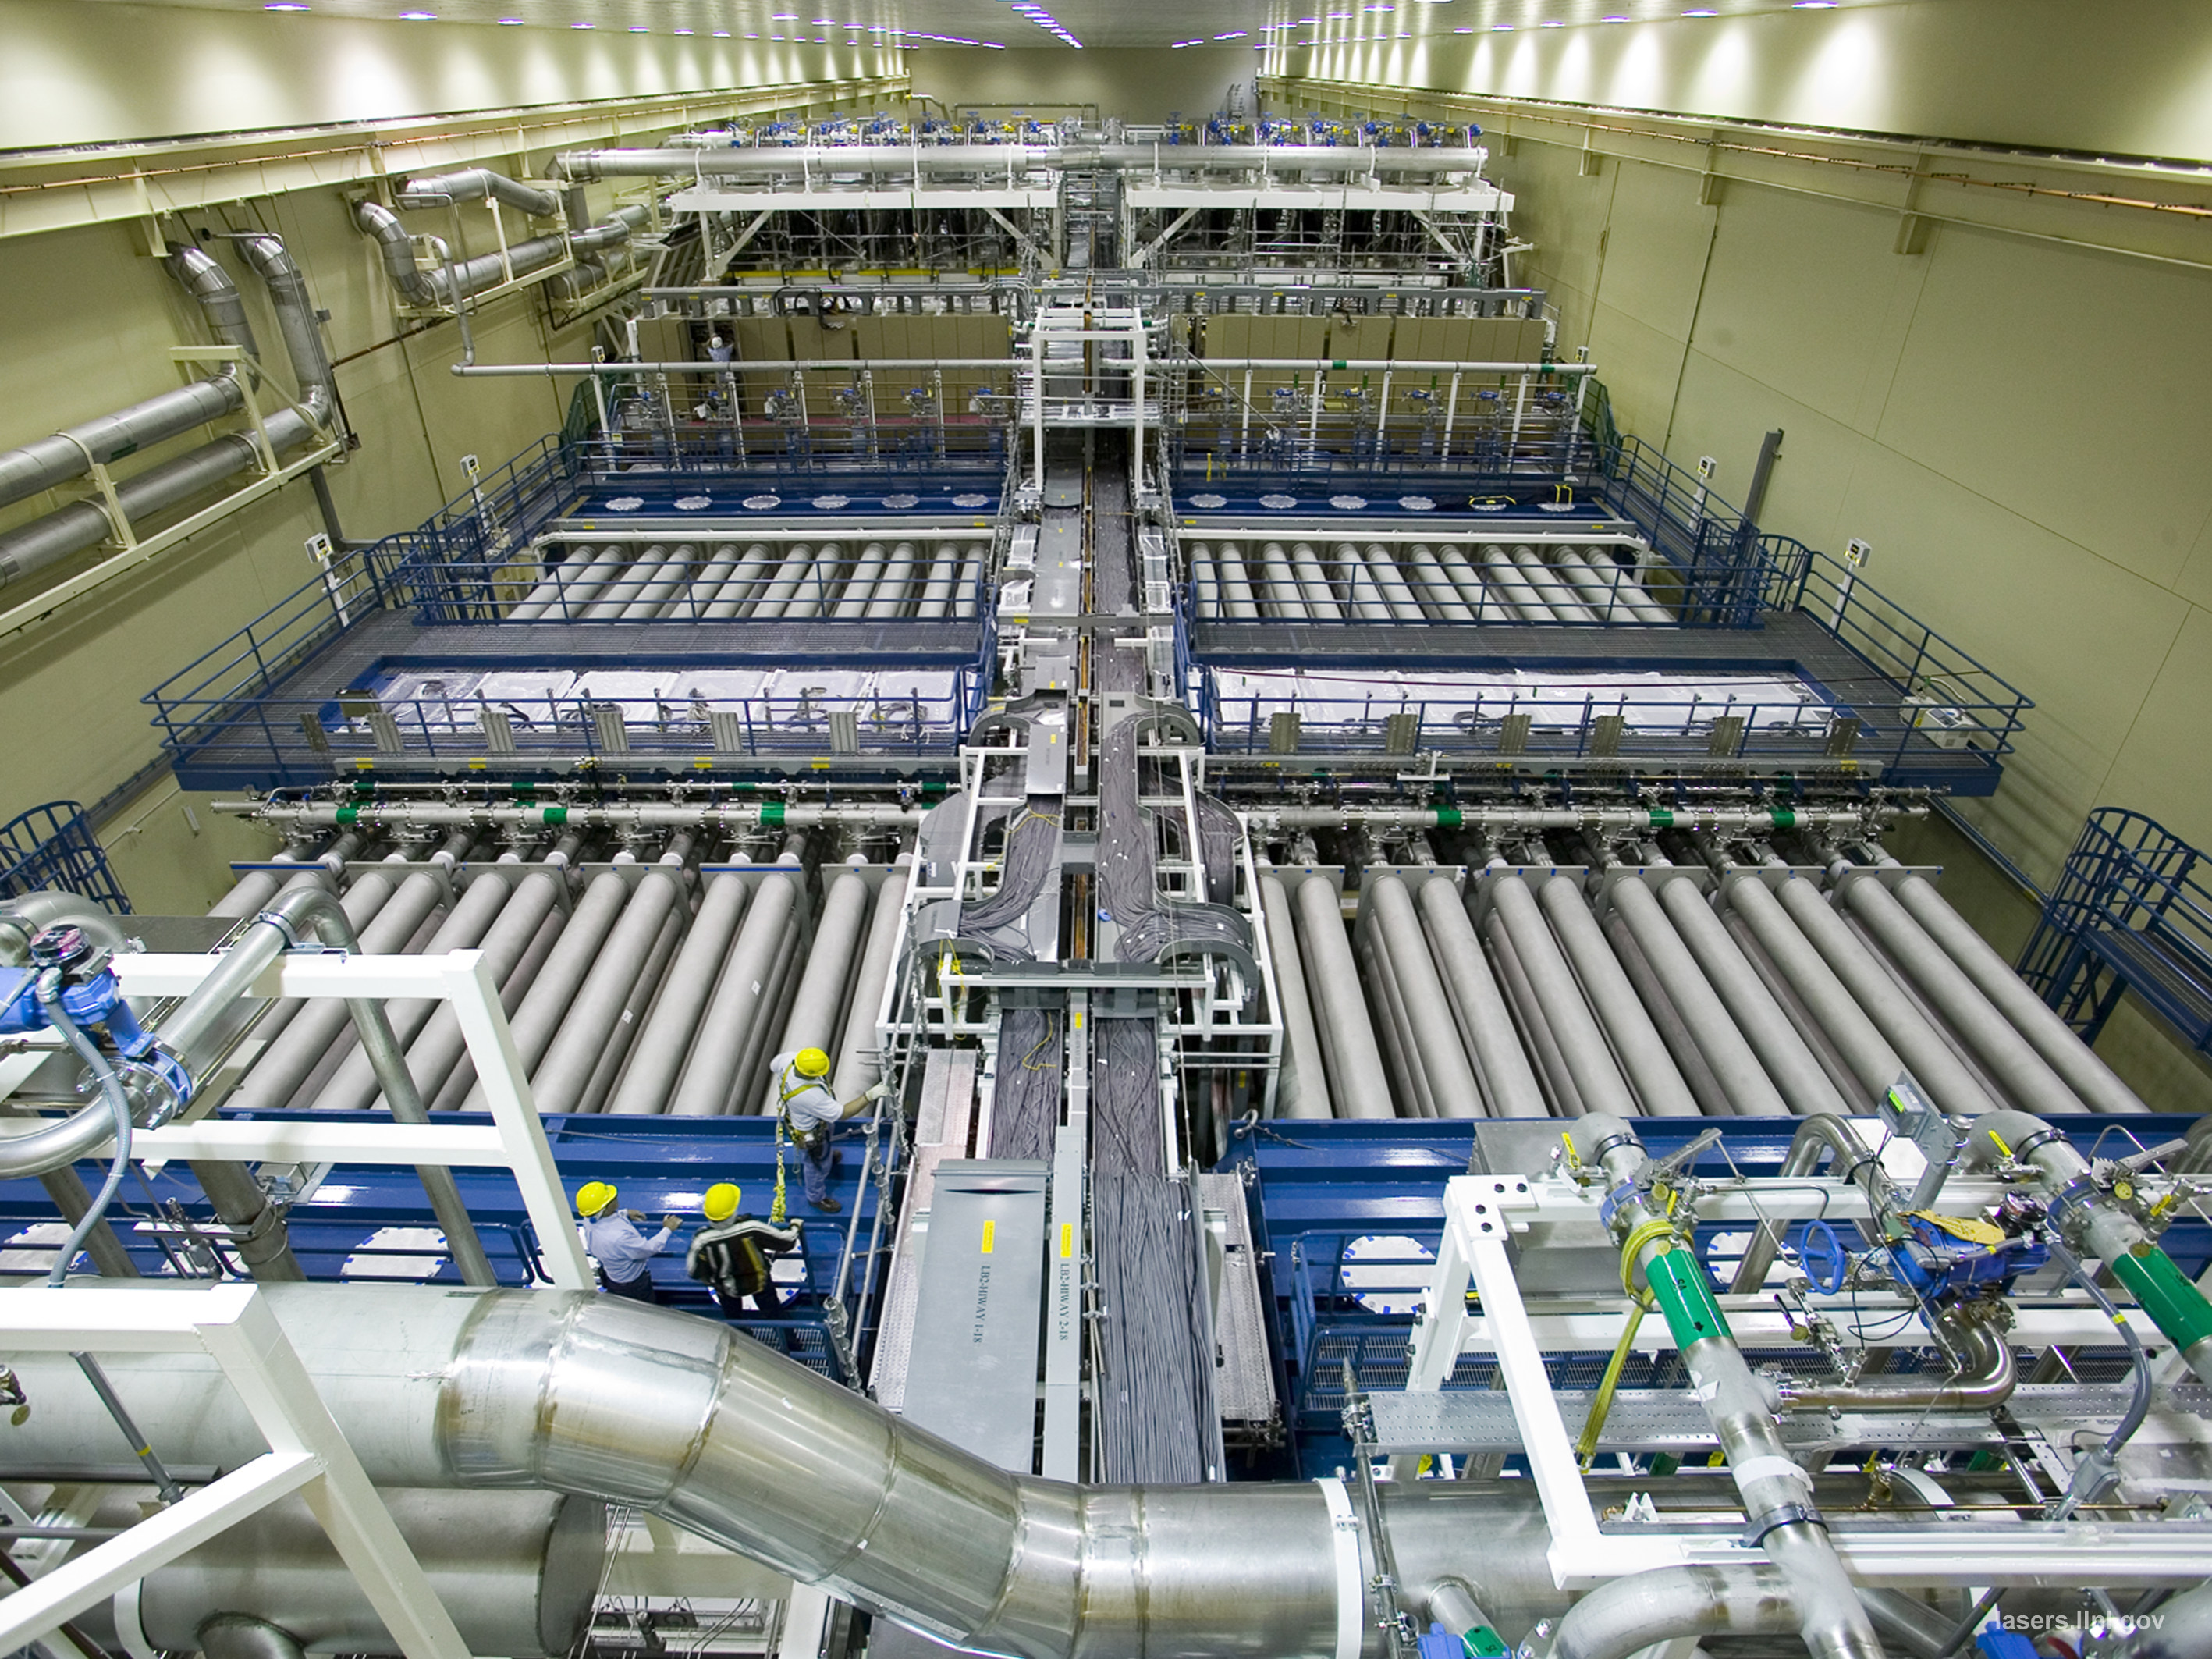
\includegraphics[width=100truemm]{slike/07_NIF_Laser_Bay.jpg}
\caption{Eden najmočnejših laserskih sistemov na svetu, ki doseže 
$500~\si{\tera\watt}$ moči v sunku. \\Vir: National Ignition Facility, Livermore, Kalifornija.}
\label{fig:NIF}
\end{figure}

Moči svetlobe, ki jih oddajajo najmočnejši laserski sistemi, imajo zelo velike
vrednosti. Najmočnejši zvezno delujoči laserji dosegajo moči prek 
$\sim 100~\si{\kilo\watt}$. Še bistveno večje moči dosegajo sunkovni laserji, 
saj lahko v sunku dosežejo moč tudi $\sim 10^{15}~\si{\watt}$. 
Vendar so sunki s tako veliko svetlobno močjo izredno kratki, tipično reda pikosekunde, tako da
znaša celotna energija v sunku ``le'' $\sim \si{\kilo\joule}$. Pomemben
parameter pri sunkovnih laserjih je tudi čas, ki poteče med dvema zaporednima
sunkoma (repeticija). Najmočnejši laserski sistemi lahko izsevajo največ nekaj sunkov dnevno. 

\section{He-Ne laser}
\index{Laser!He-Ne}
Najprej si oglejmo helij-neon (He-Ne) laser, ki je bil prvi zvezno 
delujoči laser in je še danes zelo razširjen. Najpogosteje deluje 
pri valovni dolžini $632,8~\si{\nano\metre}$ v rdečem delu spektra, lahko 
pa tudi pri infrardečih $1,15~\si{\micro\metre}$ in 
$3,39~\si{\micro\metre}$ ter nekaterih drugih\index{Infrardeče valovanje}
valovnih dolžinah v oranžnem in zelenem delu spektra. Laser deluje v zveznem 
načinu delovanja s tipičnimi močmi $0,5 - 100~\si{\milli\watt}$.

Ojačevalno sredstvo je plin, mešanica helija in neona, katerih relevantni
energijski nivoji so prikazani na sliki~(\ref{fig:HeNeE}). 
\index{Energijski nivoji!He-Ne}
\index{Trinivojski sistem}
Atome helija
s trki z elektroni vzbudimo v eno izmed dveh dolgoživih metastabilnih stanj $2^3S$ ali
$2^1S$ z razpadnima časoma $0,1~\si{\milli\second}$ in $5~\si{\micro\second}$.
Ti dve stanji slučajno praktično sovpadata z dvema stanjema neona ($4s$ in $5s$). 
Ko heliju dodamo neon, se energija s trki 
prenese z vzbujenih helijevih atomov na atome neona, ki s tem preidejo v 
že omenjeni vzbujeni stanji. Helijevi atomi se po trku vrnejo v osnovno stanje, od koder
jih lahko ponovno vzbudimo. Prenos energije z atomov helija na atome neona s trki je 
zelo učinkovit, zato zasedenost vzbujenih neonovih stanj hitro naraste. Ko preseže 
zasedenost nižjih vzbujenih stanj v neonu, pride do obnrnjene zasedenosti. 

\begin{figure}[h]
\centering
\def\svgwidth{100truemm} 
\input{slike/07_HeNeE.pdf_tex}
\caption{Shema energijskih nivojev v He-Ne laserju. Nivoji helija so označeni
z modro in nivoji neona z zeleno, laserski prehodi pa z rdečimi barvami in pripisano
ustrezno valovno dolžino.}
\label{fig:HeNeE}
\end{figure}

Znano rdečo svetlobo He-Ne laserja z valovno dolžino $632,8~\si{\nano\metre}$ dobimo 
pri prehodu iz stanja $5s$ v eno od stanj $3p$. Pri tem je življenjski čas 
stanja $5s$ okoli $100~\si{\nano\second}$, stanja $3p$ pa okoli $10~\si{\nano\second}$, zato
se spodnji nivo s spontano emisijo hitro prazni  v metastabilno stanje $3s$. 
V njem se atomi nabirajo, saj so dipolni sevalni prehodi v osnovno stanje prepovedani,
in atomi le s trki ob steno cevi prehajajo v osnovno stanje. Da pospešimo
praznjenje nivoja $3s$ in omogočimo večjo obrnjeno zasedenost, moramo torej 
zmanjšati premer razelektritvene cevi. Zaradi gibanja atomov je spektralna 
črta Dopplerjevo razširjena\index{Dopplerjeva razširitev} ($\Delta \nu = 1,5~\si{GHz}$). 

Lasersko delovanje dobimo tudi pri prehodu iz $5s$ v stanje $4p$, pri katerem 
ima izsevana svetloba valovno dolžino $3,39~\si{\micro\metre}$. 
Ojačenje je za ta prehod celo precej večje kot za
prehod pri $632,8~\si{\nano\metre}$, deloma zaradi nižje frekvence 
(glej zvezo med Einsteinovima koeficientoma $A$ in $B$, enačba~\ref{4.27}), 
deloma pa zaradi kratke življenjske dobe spodnjega laserskega nivoja $4p$. 
Zato bi pričakovali, da bo He-Ne laser svetil v infrardečem delu in ne vidnem. 
To delno prepreči absorpcija v steklu, delno pa izgube namerno povečamo s selektivno odbojnostjo
resonatorskih zrcal, ki dvigne prag delovanja za $3,39~\si{\micro\metre}$ 
nad prag za $632,8~\si{\nano\metre}$. V laser lahko dodamo tudi
celico metana, ki infrardeč del svetlobe močno absorbira, vidnega pa ne.
Omenimo še prehode iz stanja $4s$, ki ga dosežejo neonovi atomi s trki
z vzbujenimi helijevimi atomi iz nivoja $2^3S$. Prehod $4s$ v $3p$, ki da svetlobo
pri $1,15~\si{\micro\metre}$, je bil prvi opaženi prehod v He-Ne laserjih.

Tipičen He-Ne laser je razmeroma preprosto zgrajen (sliki~\ref{fig:HeNeShema}
in \ref{fig:Iskra}).\index{Laser!zgradba}
V razelektritveni cevi (napetost  $\sim 1~\si{\kilo\volt}$), skozi
katero teče električni tok ($\sim 10~\si{\milli\ampere}$), 
se nahaja mešanica helija in neona v razmerju 
$5:1 - 10:1$. Skupni tlak v cevi je nizek, le okoli $3~\si{\milli\bar}$, 
cev pa je tipično dolga okoli $0,5~\si{\metre}$ s premerom $1-2~\si{\milli\metre}$.  
Cev na obeh straneh zapirata okni, ki sta nagnjeni za Brewstrov kot (glej enačbo~\ref{eq:Brew}), 
tako da so izgube pri odboju za eno polarizacijo kar se da majhne.
Izhodna svetloba iz laserja je zato seveda polarizirana. V manjših laserjih
so namesto Brewstrovih oken na razelektritveno cev privarjena kar
resonatorska zrcala, zaradi česar so taki laserji nepolarizirani. 
Navadno je razelektritvena cev obdana z dvema ukrivljenima zrcaloma, 
ki imata zelo veliko odbojnost za izbrano valovno dolžino.
Nekaj tipičnih podatkov za He-Ne laser je zbranih v tabeli~(\ref{tab:Ar}).
\begin{figure}[h]
\centering
\def\svgwidth{100truemm} 
\input{slike/07_HeNeShema.pdf_tex}
\caption{Shema He-Ne laserja: R -- razelektritvena cev, IZ -- izhodno zrcalo, Z -- zrcalo
z veliko odbojnostjo, B -- Brewstrovi okni}
\label{fig:HeNeShema}
\end{figure}

\begin{figure}[h]
\centering
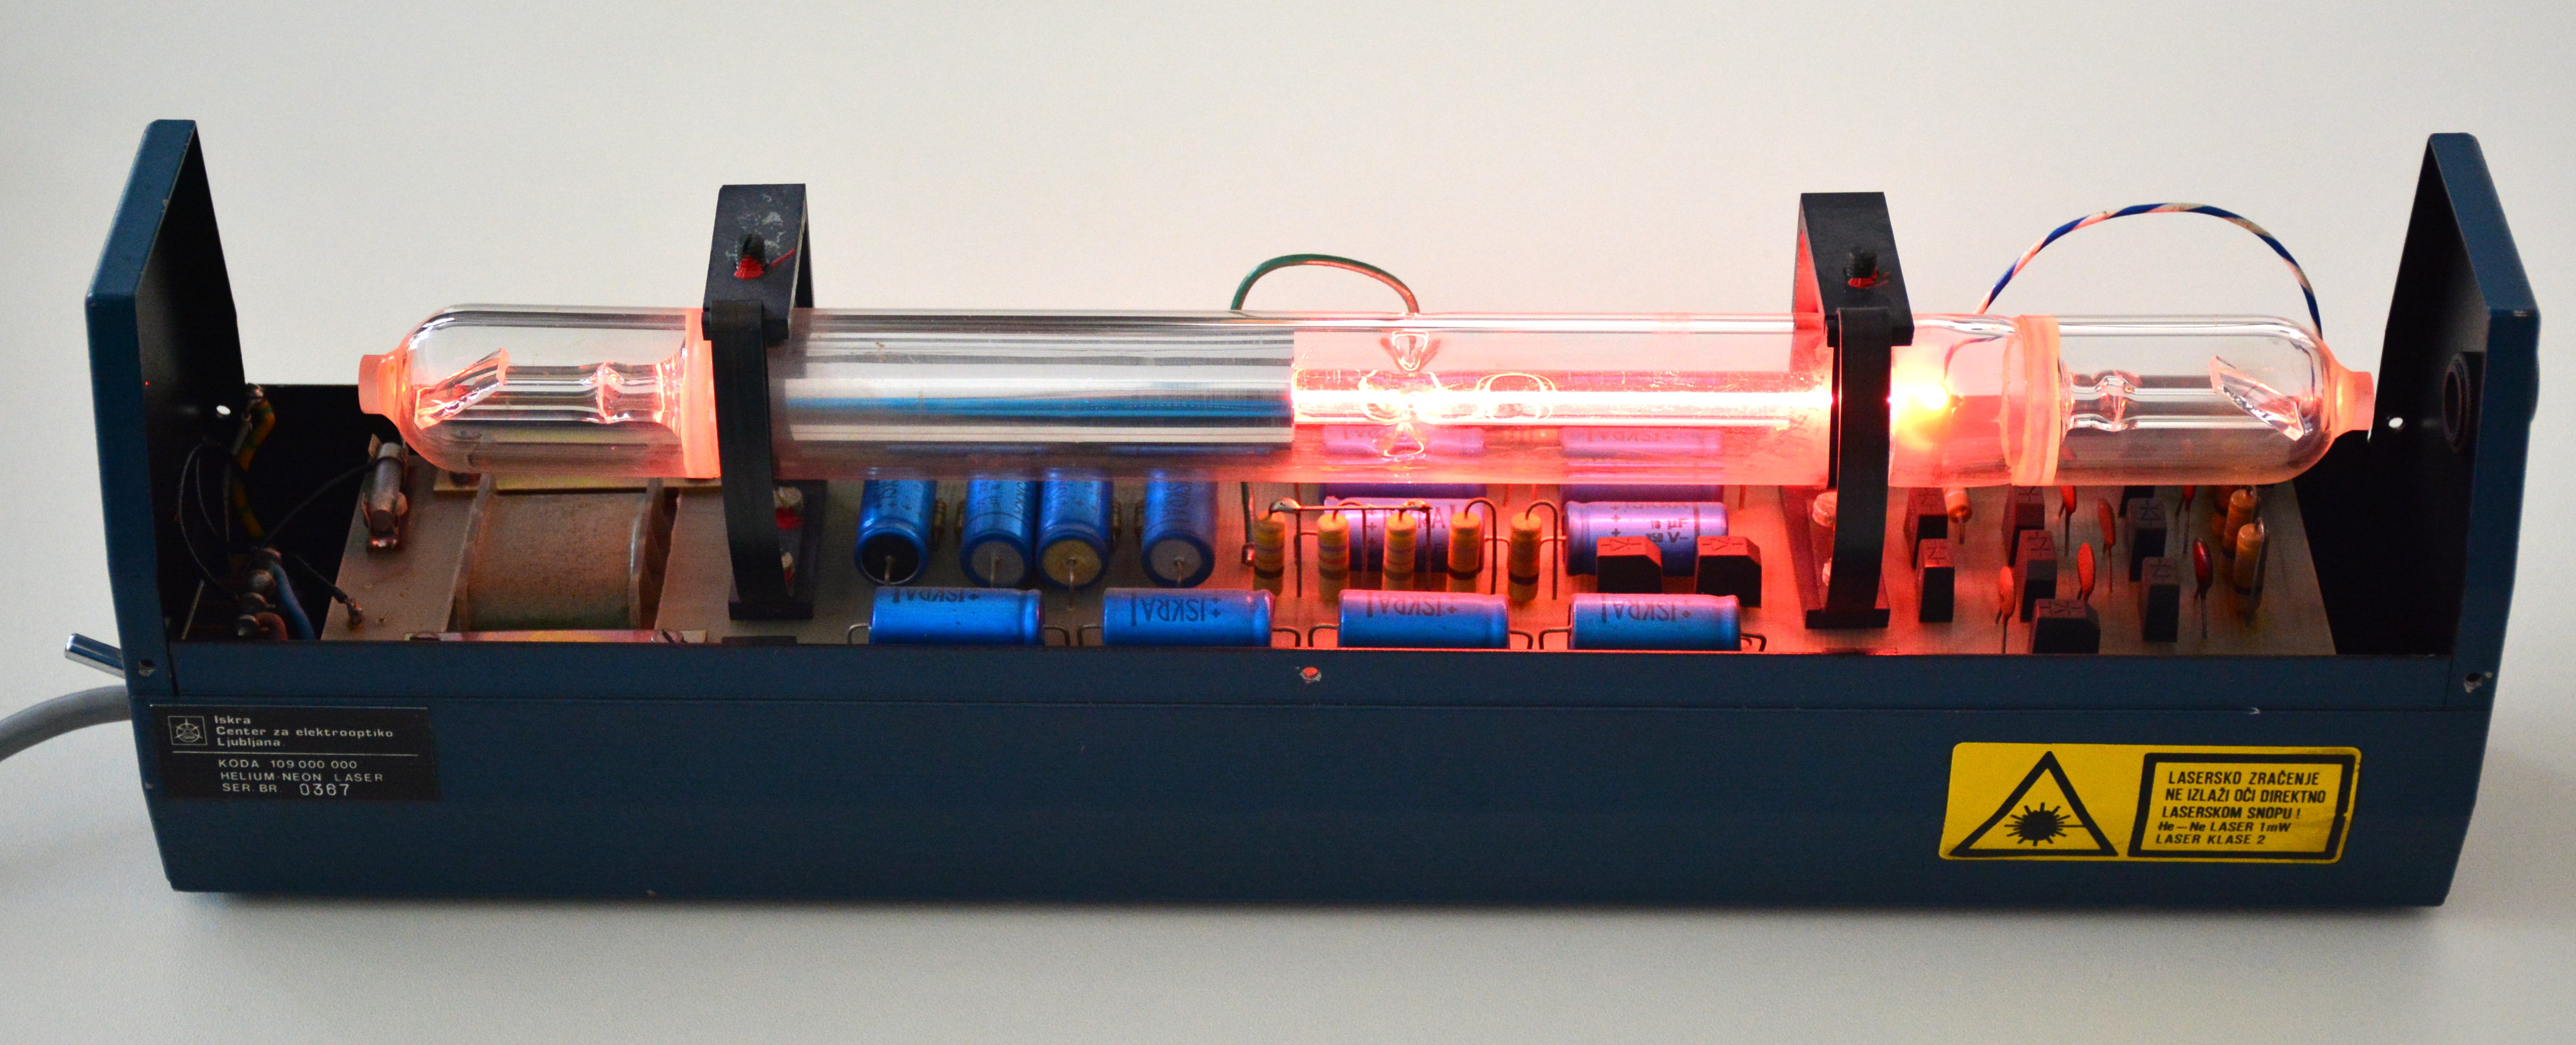
\includegraphics[width=120truemm]{slike/07_HeNe.jpg}
\caption{Primer starejšega He-Ne laserja, izdelanega v Sloveniji}
\label{fig:Iskra}
\end{figure}

He-Ne laserji so preprosti, stabilni, zanesljivi, poceni, imajo visoko kvaliteto žarka
in dolgo služijo (do 50 000 ur).
Danes jih sicer izrivajo polprevodniški laserji, vendar so še vedno v uporabi
v merilnih napravah, v optičnih čitalnih sistemih, v šolah, v raziskovalnih 
laboratorijih za interferometrijo, holografijo itd. Na njem je osnovan tudi 
standard za meter.

\section{Argonski ionski laser}
\index{Laser!argonski}
\index{Štirinivojski sistem}
Kot drugi primer plinskega laserja obravnavajmo argonski ionski (Ar$^+$) laser,
ki je najbolj poznan po zveznem delovanju v modrem in zelenem delu spektra pri 
valovnih dolžinah $488,0~\si{\nano\metre}$ in $514,5~\si{\nano\metre}$, deluje 
pa tudi v bližnjem ultravijoličnem delu spektra. Tipične moči delovanja argonskega laserja
so $100~\si{\milli\watt} - 50~\si{\watt}$.\index{Ultravijolično valovanje}

Kot večino drugih plinskih laserjev tudi tega črpamo z električnim tokom.
Atome argona vzbudimo s trki z elektroni v ione argona, ti pa z nadaljnjimi
trki preidejo v vzbujena stanja. Obrnjeno zasedenost
dosežemo med nivojema $4p$ in $4s$ (slika~\ref{fig:ArE}). 
Ta dva nivoja vsebujeta veliko podnivojev, zato je tudi prehodov med
njima zelo veliko. Argonski laser tako seva pri več kot tridesetih različnih
valovnih dolžinah, najznačilnejši sta že omenjeni 488~nm in 514,5~nm. 
Življenjski čas zgornjega nivoja $\sim 10^{-8}~\si{\second}$ je približno 
desetkrat daljši od življenjskega časa spodnjega nivoja, od koder se ioni
z rekombinacijo z elektroni vrnejo v osnovno stanje atoma. Tudi pri tem laserju
je poglavitni vzrok za razširitev črte \index{Dopplerjeva razširitev}Dopplerjev 
pojav.\index{Energijski nivoji!argon}

\begin{figure}[h]
\centering
\def\svgwidth{80truemm} 
\input{slike/07_ArE.pdf_tex}
\caption{Shema energijskih nivojev v Ar$^+$ laserju}
\label{fig:ArE}
\end{figure}

Argonski laser je v osnovi zgrajen podobno kot He-Ne laser. \index{Laser!zgradba}
V razelektritveni cevi
(tipična dolžina $1~\si{\metre}$ in premer $1-2~\si{\milli\metre}$)
se nahaja argon pri pritisku okoli $10~\si{\milli\bar}$. Ker gre pri 
vzbujanju atomov argona za dvostopenjski proces, mora biti električni tok, 
s katerim dosežemo obrnjeno zasedenost, precej velik, lahko tudi nekaj deset amperov. 
Pri tipični napetosti nekaj kV to pomeni, da so potrebne velike električne moči, 
pogosto več deset $\si{\kilo\watt}$, in močnejši argonski laserji so zato zaradi 
velike količine odvečne toplote najpogosteje vodno hlajeni.

\begin{figure}[h]
\centering
\def\svgwidth{110truemm} 
\input{slike/07_ArShema.pdf_tex}
\caption{Poenostavljena shema Ar laserja s prizmo: R -- razelektritvena cev, 
IZ -- izhodno zrcalo, Z -- zrcalo z veliko odbojnostjo, B -- Brewstrovi okni, 
P -- prizma
}
\label{fig:ArS}
\end{figure}

V argonskih laserjih pogosto ustvarimo tudi vzdolžno magnetno polje, ki preprečuje 
elektronom, da bi predčasno zapustili ojačevalno območje in trčili v steno. S
tem se poveča izhodna moč laserja, hkrati pa preprečuje poškodbe na stenah, ki bi jih 
lahko povzročili visokoenergijski elektroni. Iz istega razloga so pri močnejših
laserjih zrcala izven plinske cevi. 

V resonator argonskega laserja pa moramo vgraditi še en dodaten element, ki omogoči
izbiro ene same spektralne črte. Najpogosteje za ta frekvenčno selektiven element
uporabimo kar majhno prizmo pred enim od obeh zrcal (slika~\ref{fig:ArS}). Zaradi disperzije
v prizmi se snopi različnih valovnih dolžin lomijo pod različnimi koti in le tisti 
snop, ki vpada pravokotno na zrcalo, je ojačen. Z vrtenjem prizme ali zrcala lahko 
tako izberemo valovno dolžino ojačene svetlobe. Nekaj tipičnih podatkov za argonski
laser je zbranih v tabeli~(\ref{tab:Ar}).

Argonski laser je zanesljiv in daje zelo kvaliteten osnovni Gaussov snop pri eni
sami frekvenci. Zato se dosti uporablja v optični spektroskopiji,
interferometriji, holografiji in merilni tehniki. Deluje lahko v zveznem načinu,
zaradi razmeroma široke črte ojačenja pa ga uporabljamo tudi za fazno uklenjen
sunkovni laser z dolžino sunkov okoli $150~\si{\pico\second}$. 
V kombinaciji s kriptonovim laserjem, ki je zelo podoben argonskemu, le da deluje
v rdečem in oranžnem delu spektra, se uporablja tudi v zabavni industriji.
V zadnjem času ga vse bolj izrivajo polprevodniški laserji ali pa frekvenčno
podvojeni Nd:YAG. 

\section{Laser na ogljikov dioksid}
\index{Laser!CO$_2$}
Do zdaj opisani laserji so delovali na elektronskih prehodih v atomih oziroma ionih. 
Laser na ogljikov dioksid pa deluje na prehode med vibracijskimi stanji molekul 
CO$_2$, pri čemer elektroni ostanejo v osnovnem stanju.
Zaradi majhnih energijskih razlik med vibracijskimi stanji deluje
tak laser v infrardečem delu spektra, najpogosteje pri \index{Infrardeče valovanje}
$9,6~\si{\micro\metre}$ in $10,6~\si{\micro\metre}$. Laser deluje v zveznem
in v sunkovnem načinu, odlikuje ga pa zelo velik izkoristek ($~\sim 30~\%$) in 
posledično zelo velike moči, $1~\si{\watt} - 10~\si{\kilo\watt}$. 

Preden opišemo delovanje laserja, si na kratko oglejmo še nihajna stanja molekule 
ogljikovega dioksida. Molekula CO$_2$ je v osnovnem stanju linearna molekula 
(slika~\ref{fig:CO2}\,a). 
Za molekule take oblike obstajajo trije osnovni načini nihanja atomov glede na težišče:
atoma kisika nihata simetrično vzdolž osi molekule, pri čemer ogljik miruje --
simetrični razteg (slika~\ref{fig:CO2}\,b), atomi nihajo v smeri pravokotno na 
os -- upogib (slika~\ref{fig:CO2}\,c) in atoma kisika se gibljeta v isti smeri 
vzdolž osi, ogljik pa v nasprotni smeri -- asimetrični razteg (slika~\ref{fig:CO2}\,d). 
Pri tem ima najvišjo frekvenco asimetrični razteg, najnižjo pa upogib. 
Vsako vibracijsko stanje lahko razstavimo na osnovne nihajne načine in 
ga opišemo s številom energijskih kvantov v posameznem osnovnem nihanju, 
torej s trojico celih števil $(n_1,n_2,n_3)$. Stanje 100 tako opisuje
osnovni simetrični razteg, stanje 010 osnovno upogibno nihanje, stanje 001 pa 
osnovni asimetrični razteg.

\begin{figure}[h]
\centering
\def\svgwidth{100truemm} 
\input{slike/07_CO2.pdf_tex}
\caption{Molekula CO$_2$ (a) in trije osnovni načini nihanja molekule:
simetrični razteg (b), upogib (c) in asimetrični razteg (d)}
\label{fig:CO2}
\end{figure}

Vibracijska stanja molekule vzbudimo z električnim tokom skozi plin. 
\index{Energijski nivoji!CO$_2$}
\index{Štirinivojski sistem}
Pri tem v razelektritveno cev dodamo dušik (N$_2$) in podobno kot pri He-Ne laserju
se tudi CO$_2$ črpa predvsem preko trkov z dušikovimi molekulami. 
Dušikova molekula je dvoatomna in ima zato zgolj eno vibracijsko stanje, ki po energiji
praktično sovpada z energijo stanja 001 (slika~\ref{fig:CO2E}). Iz tega gornjega
stanja prehajajo molekule v stanje 100 ($10,6~\si{\micro\metre}$) ali v stanje
020 ($9,6~\si{\micro\metre}$). Da pospešimo prehod nazaj v osnovno stanje, 
plinski mešanici dodamo še helij, s katerim trkajo molekule.
Razmerje parcialnih tlakov je tako navadno 1:1:8 za CO$_2$:N$_2$:He pri tlaku $1~\si{\milli\bar}$. 
Pri tako nizkih tlakih je poglavitna razširitev spektralne črte Dopplerjeva, 
\index{Dopplerjeva razširitev}ki 
pa je v primerjavi z ostalimi plinskimi laserji zaradi nizih frekvenc zelo majhna,
le okoli $70~\si{\mega\hertz}$. V laserskih sistemih, kjer je tlak plinov večji,
prevlada razširitev zaradi medmolekulskih trkov. Pri tlakih okoli $20~\si{\bar}$
znaša razširitev že okoli $500~\si{\giga\hertz}$, kar omogoča izdelavo fazno uklenjenih 
sunkovnih laserjev s sunki dolžine $\sim 1~\si{\pico\second}$. Nekaj tipičnih podatkov 
za laser na ogljikov dioksid je zbranih v tabeli~(\ref{tab:Ar}).

\begin{figure}[h]
\centering
\def\svgwidth{95truemm} 
\input{slike/07_CO2E.pdf_tex}
\caption{Shema vibracijskih nivojev v CO$_2$ laserju}
\label{fig:CO2E}
\end{figure}

Najpreprostejši laser na ogljikov dioksid \index{Laser!zgradba} 
je po svoji zgradbi podoben že obravnavanim plinskim laserjem. 
Razelektritvena cev (polmer $\sim 1~\si{\centi\metre}$ in dolžina $0,5-2~\si{\metre}$) 
je na obeh koncih zaključena z Brewstrovima oknoma in zrcaloma, pri čemer moramo paziti,
da elementi prepuščajo oziroma odbijajo infrardeč del svetlobe. Ker lahko deluje
laser pri zelo veliko različnih valovnih dolžinah, dodamo frekvenčno selektiven
člen, na primer uklonsko mrežico (slika~\ref{fig:CO2S}).\index{Uklonska mrežica}

\begin{figure}[h]
\centering
\def\svgwidth{100truemm} 
\input{slike/07_CO2Shema.pdf_tex}
\caption{Poenostavljena shema najpreprostejšega CO$_2$ laserja: R -- razelektritvena cev, 
IZ -- izhodno zrcalo, Z -- zrcalo z veliko odbojnostjo, B -- Brewstrovi okni, 
U -- uklonska mrežica
}
\label{fig:CO2S}
\end{figure}

Poleg običajnih zaprtih sistemov poznamo tudi laserje z vzdolžnim ali prečnim pretokom, 
valovodne laserje ... Razlikujejo se po svojih specifikacijah in vrsti uporabe.
Laserji na ogljikov dioksid se največ uporabljajo v industriji za zahtevne 
obdelave materialov, na primer za rezanje 
kovin, vrtanje, ablacijo, varjenje, pa tudi za vojaške in medicinske namene.
Obdelava z laserji omogoča veliko natančnost, čistočo in je zelo fleksibilna.

\begin{table}
\small
\begin{center}
\begin{tabular}{|l|c|c|c|c|}\hline
Laser & He-Ne & Ar$^+$ & CO$_2$ & ekscimer\\ \hline
Valovna dolžina  $\lambda$ & $632,8~\si{\nano\metre}$& $488$ in
$514,5~\si{\nano\metre}$ & $9,6$ in $10,6~\si{\micro\metre}$ & UV
\\ \hline
Verjetnost za spontani prehod $A$ & $3,4 \times 10^6/\si{\second}$ & 
$7,8 \times 10^7/\si{\second}$ & $0,25/\si{\second}$ & $\sim 10^8/\si{\second}$ \\ \hline
Presek za stimulirano emisijo $\sigma$ & $3 \times 10^{-17}~\si{\metre}^2$&  $2,6 \times 10^{-16}~\si{\metre}^2$ & $3 \times 10^{-22}~\si{\metre}^2$ & $ 10^{-20}~\si{\metre}^2$ \\ \hline
Spektralna širina črte $\Delta \nu$ & $1,5 \times 10^{9}~\si{\hertz}$ & 
$3,5 \times 10^{9}~\si{\hertz}$ &$7 \times 10^{7}~\si{\hertz}$ & $10^{13}~\si{\hertz}$ \\ \hline
Obrnjena zasedenost $\Delta N/V$ & $5 \times 10^{15}/\si{\metre}^3$ & $2 \times 10^{15}/\si{\metre}^3$ & $3 \times 10^{21}/\si{\metre}^3$ & $10^{20}/\si{\metre}^3$\\ \hline
\end{tabular}
\caption{Izbrani podatki za He-Ne, Ar$^+$, CO$_2$ in tipičen ekscimerni laser}
\index{Laser!He-Ne}
\index{Laser!argonski}
\index{Laser!CO$_2$}
\index{Laser!ekscimerni}
\label{tab:Ar}
\end{center}
\end{table}

\section{Ekscimerni laser}
\index{Laser!ekscimerni}
Ekscimerji ({\it excited dimer, excimer}) so vzbujena vezana stanja dveh atomov, 
ki bi se v osnovnem stanju ne vezala. Za laserje so zanimivi predvsem ekscimerji
težkih žlahtnih plinov in halogenov, na primer Ar$_2^*$ ($126~\si{\nano\metre}$), 
Kr$_2^*$ ($146~\si{\nano\metre}$), Xe$_2^*$ ($172~\si{\nano\metre}$),
ArF ($193~\si{\nano\metre}$), KrF ($248~\si{\nano\metre}$), 
XeCl ($308~\si{\nano\metre}$), ArBr ($161~\si{\nano\metre}$), 
NeF ($108~\si{\nano\metre}$) ... Te molekule obstajajo samo v vzbujenem stanju,
v osnovnem stanju pa je odbojna sila med atomoma prevelika in molekula neobstojna.
Vsi našteti primeri oddajajo lasersko svetlobo v\index{Ultravijolično valovanje}
ultravijoličnem delu, ki ga drugi laserski sistemi le težko pokrivajo. 
Ekscimerni laserji delujejo v sunkih, pri čemer je tipična oddana energija v sunku 
$\sim 1~\si{\joule}$, dolžina sunka $10-100~\si{\nano\second}$ in repeticija 
$\sim 100~\si{\hertz}$.

Vezano stanje dveh atomov dobimo, kadar je ionizacijska energija prvega
atoma manjša od vsote elektronske afinitete drugega atoma in
elektrostatične energije vezave obeh ionov. Vzemimo za primer klor in
kripton. Ionizacijska energija kriptona v osnovnem stanju je 14~eV, v
vzbujenem pa 5~eV. Elektronska afiniteta klora je 3,75~eV in
elektrostatična vezavna energija KrCl okoli 7~eV. Tako je za nastanek
molekule KrCl v osnovnem stanju potrebno dodati okoli 4~eV, pri tvorbi
molekule v vzbujenem stanju pa se sprosti okoli 6~eV. Približno obliko
celotne potencialne energije molekule KrCl v osnovnem in vzbujenem stanju
kaže slika~(\ref{fig:exE}). Molekula, ki je vezana v vzbujenem stanju, po
sevalnem prehodu v osnovno stanje takoj razpade, zato je zelo lahko doseči
obrnjeno zasedenost. Pri tem je razpadni čas vezanega stanja $\sim~10~\si{\nano\second}$,
spodnjega nevezanega pa okoli $0,1~\si{\pico\second}$.
Spektralna širina prehoda je precej velika, okoli $1~\si{\nano\metre}$.
Da nastanejo ekscimeri, vzbujamo mešanico 
plinov (žlahtnega plina ali mešanice žlahtnega in halogenega plina) v heliju. Ker je pritisk
razmeroma velik (npr. 2 ali $3~\si{\bar}$), je vzbujanje prečno, podobno kot pri 
nekaterih izvedbah CO$_2$ laserja. Nekaj tipičnih podatkov 
za ekscimerni laser je zbranih v tabeli~(\ref{tab:Ar}).
\index{Energijski nivoji!ekscimer}

Ekscimerni laserji delujejo v sunkih s precej veliko energijo in se uporabljajo 
v industriji materialov, mikroprocesorjev, fotolitografiji in medicini, predvsem 
oftalmologiji in kirurgiji.
\begin{figure}[h]
\centering
\def\svgwidth{50truemm} 
\input{slike/07_exE.pdf_tex}
\caption{Shema energije v odvisnosti od razdalje med jedroma atomov. V vzbujenem stanju
se atoma povežeta v molekulo, po prehodu v nižji nivo pa atoma disociirata.}
\label{fig:exE}
\end{figure}


\section{Neodimov laser}
Druga skupina laserjev so trdninski laserji. Taki laserji
so osnovani na elektronskih prehodih v ionih primesi, ki jih dodamo v kristal ali steklo,
črpamo pa jih optično. Primesi so praviloma redke zemlje ali prehodne kovine, 
kristali pa so navadno oksidi ali fluoridi. Izdelava ojačevalnih sredstev na osnovi stekla
je bistveno bolj preprosta in poceni, vendar ima steklo precej nižjo toplotno prevodnost
od kristalov in se zato bolj greje. 
Začeli bomo z opisom dveh primerov neodimovega laserja, Nd:YAG in Nd:steklo. Podobne laserje dobimo, 
če v YAG kristalu namesto z neodimom itrijeve ione nadomestimo z iterbijem ($1030~\si{\nano\metre}$) ali erbijem ($2940~\si{\nano\metre}$).

\subsection{Nd:YAG}
\index{Laser!Nd:YAG}
Najpomembnejši predstavnik je Nd:YAG laser, v katerem je ojačevalno sredstvo
itrij-aluminijev granat (Y$_3$Al$_5$O$_{12}$, YAG) s primesmi neodimovih ionov Nd$^{3+}$. 
Neodimov laser deluje pri valovni dolžini $1,064~\si{\micro\meter}$ ali frekvenčno podvojeni
$532~\si{\nano\metre}$. Laser lahko deluje v zveznem 
načinu pri močeh $5-100~\si{\watt}$ ali sunkovnem z dolžino sunkov okoli 
$100~\si{\nano\second}$ in energijo sunka $\sim 1~\si{\joule}$.

Neodimov laser je primer štirinivojskega laserskega sistema, 
\index{Štirinivojski sistem}pri čemer je 
laserski prehod med stanjema $^4$F$_{3/2}$ in $^4$I$_{11/2}$ iona neodima 
(slika~\ref{fig:NdE}). S svetlobo višje frekvence 
(tipično okoli $800~\si{\nano\metre}$) črpamo elektrone v višje nivoje, ki hitro 
preidejo v zgornji laserski nivo. Življenjski čas višjega nivoja je 
okoli $230~\si{\micro\second}$, spodnjega pa precej krajši, zato je 
lahko doseči veliko obrnjeno zasedenost. Spodnje stanje je dovolj visoko nad 
osnovnim, da pri sobni temperaturi v ravnovesju ni znatno zasedeno. Zato je 
prag neodimovega laserja nizek in je lahko doseči zvezno stacionarno delovanje, 
prav tako dobro pa deluje tudi v sunkih. Razširitev črte je homogena in je predvsem posledica
termičnega nihanja kristalne mreže. Laser je odličen za delovanje s preklopom dobrote, 
zaradi ozke črte pa z uklepanjem faz oddaja zelo kratke sunke (nekaj ps). 
\index{Energijski nivoji!Nd:YAG}
\begin{figure}[h]
\centering
\def\svgwidth{85truemm} 
\input{slike/07_NdE.pdf_tex}
\caption{Shema energijskih nivojev v Nd$^{3+}$ laserju}
\label{fig:NdE}
\end{figure}

Za črpanje uporabljamo diodne laserje ali močne ksenonove svetilke za zvezno delovanje 
ter podobne bliskovne luči za sunkovno delovanje (slika~\ref{fig:Nd}\,a). 
Aktivna snov v laserju je v obliki paličice dolžine od nekaj cm do dobrih 
$10~\si{\centi\metre}$ in širine do okoli $1~\si{\centi\metre}$. 
V kristalu YAG neodimovi ioni nadomestijo približno $1~\%$ itrijevih, zato ojačevalno
sredstvo na videz ni prozorno, temveč rahlo rožnato (slika~\ref{fig:Nd}\,b). 
Aktivna paličica in svetilka sta vgrajeni v cilindrično ali eliptično votlino z 
zrcalnimi ali belimi stenami, tako da se čim večji del črpalne svetlobe absorbira v 
laserski paličici (slika~\ref{fig:Nd}\,c).

\begin{figure}[h]
\centering
\def\svgwidth{120truemm} 
\input{slike/07_Nd.pdf_tex}
\caption{Ksenonska bliskovna svetilka (a), ojačevalno sredstvo v Nd:YAG laserju (b) 
in shema eliptične črpalne votline (c)}
\label{fig:Nd}
\end{figure}

Pri črpanju s ksenonsko svetilko je le manjši del izsevane svetlobe v
absorpcijskih pasovih, zato je izkoristek črpanja razmeroma slab, tipično 
pod $0,01~\%$. Za izhodno moč zvezno delujočega Nd:YAG laserja nekaj deset wattov je tako
potrebna električna moč nekaj kW. Velika večina porabljene moči 
gre v gretje, zato je v laserjih z nekoliko večjo povprečno
močjo potrebno vodno hlajenje. Gretje povzroča tudi toplotne deformacije
laserske paličice, kar lahko močno spremeni lastnosti resonatorja. Toplotni
učinki so ena poglavitnih praktičnih težav pri izdelavi neodimovih
laserjev s klasičnimi svetilkami . Danes prevladuje
 črpanje z diodnimi laserji, ki svetijo v območju največje
absorpcije Nd$^{3+}$. Črpanje je lahko prečno ali pa vzdolžno (slika~\ref{fig:NdS}). 
Pri diodnem črpanju je izkoristek dosti večji in je manj gretja, kar omogoča 
bolj kompaktno konstrukcijo in boljšo stabilnost izhodne moči.
\index{Laser!zgradba} 
\begin{figure}[h]
\centering
\def\svgwidth{120truemm} 
\input{slike/07_NdS.pdf_tex}
\caption{Shema vzdolžnega diodnega črpanja Nd:YAG laserja. O -- ojačevalno sredstvo, 
IZ -- izhodno zrcalo, D -- dikroično zrcalo, 
prepustno za črpalno svetlobo in odbojno za lasersko, DL -- diodni 
laser za črpanje, L -- leča
}
\label{fig:NdS}
\end{figure}

Neodimovi laserji so zelo razširjeni, tako v osnovni kot tudi v frekvenčno 
podvojeni različici. 
Najbolj uporabni so za obdelavo materialov (na primer vrtanje in varjenje, 
litografija) ter v medicini (dermatologija in endoskopska kirurgija). 
Pomemben proizvajalec Nd:YAG laserjev 
za medicinske namene je tudi podjetje Fotona iz Ljubljane. 

\begin{table}[h]
\small
\begin{center}
\begin{tabular}{|l|c|c|c|}\hline
Laser & Nd:YAG & Nd:steklo & Ti:safir \\ \hline
Valovna dolžina  & $1064~\si{\nano\metre}$ & $1050~\si{\nano\metre}$ & 
 $660-1180~\si{\nano\metre}$\\ \hline
Verjetnost za spontani prehod $A$ & $4 \times 10^3/\si{\second}$ & $3 \times 10^3/\si{\second}$
& $3 \times 10^5/\si{\second}$\\ \hline
Presek za stimulirano emisijo $\sigma$ & $3 \times 10^{-23}~\si{\metre}^2$ &
$3 \times 10^{-24}~\si{\metre}^2$ & $3 \times 10^{-23}~\si{\metre}^2$\\ \hline
Spektralna širina črte $\Delta \nu$ & $1,3 \times 10^{11}~\si{\hertz}$ &
$7 \times 10^{12}~\si{\hertz}$ & $1 \times 10^{14}~\si{\hertz}$\\ \hline
Gostota obrnjene zasedenosti $\Delta N/V$ & $1,6 \times 10^{23}/\si{\metre}^3$ &
$8 \times 10^{23}/\si{\metre}^3$ & $6 \times 10^{23}/\si{\metre}^3$\\ \hline
\end{tabular}
\caption{Tipični podatki za Nd:YAG, Nd:steklo in Ti:safirni laser}
\index{Laser!Nd:YAG}
\index{Laser!Nd:steklo}
\index{Laser!Ti:safir}
\label{tab:nd}
\end{center}
\end{table}

\subsection{Nd:steklo}
\index{Laser!Nd:steklo}
Namesto v ustrezen kristal lahko neodimove ione Nd$^{3+}$ vgradimo tudi v steklo. 
Tak laser deluje pri valovni dolžini $1,050~\si{\micro\meter}$ v sunkovnem načinu 
s preklopom dobrote ali z uklepanjem faz z energijami sunkov $~\sim 1~\si{\joule}$.
Z ojačevalniki dosežemo energije sunka nad $100~\si{\kilo\joule}$. 
Zaradi amorfne strukture stekla in posledično 
nehomogenega lokalnega polja je laserska črta nehomogeno razširjena.
\index{Spektralna črta!nehomogena razširitev}
Ojačenje je manjše kot v Nd:YAG in za prag laserskega delovanja je
potrebna precej večja moč črpanja. Laserji Nd:steklo zato delujejo le v sunkovnem
načinu, kjer pa so za velike energije celo boljši od Nd:YAG. Zaradi
manjšega ojačenja pri dani obrnjeni zasedenosti je v laserju s preklopom
dobrote mogoče doseči večjo načrpanost, ne da bi prišlo do praznjenja
zaradi ojačevanja spontanega sevanja v enem preletu paličice. Problem teh laserjev
predstavlja nizka toplotna prevodnost stekla, ki omejuje repeticijo sunkov.
Velika širina črte je zelo primerna za delovanje v načinu uklepanja faz, s 
katerim dosegamo ultrakratke sunke ($\sim 100~\si{\femto\second}$). 

\begin{remark}
Energije izsevanih sunkov je mogoče še povečati z ojačevalniki. Med največjimi je
laserski sistem Nd:steklo v Rochestru (New York), ki ga uporabljajo
za raziskave fuzije. Okoli $1~\si{\nano\second}$ dolg sunek iz osnovnega laserja razdelijo na
deset ojačevalnih vej, ki so dolge po $180~\si{\metre}$.
Končna energija sunka je nad $\sim 1~\si{\mega\joule}$. Z njim z vseh strani posvetijo na
kroglico iz devterija in tritija, ki se dovolj segreje in stisne, da pride
do njunega zlivanja. Vršna moč laserskega sunka je okoli $10^{15}$~W. 
Če laserski snop zberemo na površino 1~mm$^2$, dobimo električno poljsko jakost
okoli $5 \times 10^{11}$~V/m, kar je približno enako polju v vodikovem atomu.
\end{remark}

\section{Titan-safirni laser}
\index{Laser!Ti:safir}
Titan-safirni laser (Ti:safir) je trdninski laser, pri katerem so v kristal safirja
Al$_2$O$_3$ primešani ioni titana Ti$^{3+}$. Njegova najpomembnejša značilnost je
zvezna nastavljivost valovne dolžine v zelo širokem frekvenčnem pasu 
($600-1180~\si{\nano\metre}$) z največjo učinkovitostjo pri okoli $800~\si{\nano\metre}$. Deluje
v zveznem načinu z močmi do $50~\si{\watt}$ in v fazno uklenjenem načinu sunkovno 
z dolžino sunkov do $10~\si{\femto\second}$ z vršnimi močmi nad $10^{12}~\si{\watt}$. 
\index{Energijski nivoji!Ti:safir}
\begin{figure}[h]
\centering
\def\svgwidth{90truemm} 
\input{slike/07_TiE.pdf_tex}
\caption{Energijski nivoji v titan-safirnem laserju. Dva nivoja sta zaradi vibracij
razcepljena na veliko število podnivojev, ki pa se med seboj deloma prekrivajo.
Zelo podobna je tudi shema energijskih nivojev organskih barvil. 
}
\label{fig:TiE}
\end{figure} 

Ojačevalno sredstvo v titan-safirnem laserju je aluminijev oksid, v katerem 
približno $0,2~\%$ aluminijevih ionov nadomestimo s titanovimi. Titanovi ioni imajo 
v taki konfiguraciji zgolj eno vzbujeno stanje, vendar se zaradi sklopitve s fononi
vibracijski nivoji posameznega stanja med seboj prekrivajo in prehod je močno razširjen. 
Z optičnim črpanjem vzbudimo titanov ion iz osnovnega stanja v eno izmed vibracijskih 
stanj vzbujenega stanja, ki hitro preide v najnižje vzbujeno stanje. 
Laserski prehod poteka med nižjem vzbujenim stanjem in enim od vibracijskih 
nivojev osnovnega stanja (slika~\ref{fig:TiE}), od koder se vrne v osnovno stanje. Življenjski čas
vzbujenega stanja je kratek ($3,2~\si{\micro\second}$), širina črte pa največja med
vsemi trdninskimi laserji. Ker je vrh absorpcijskega pasu blizu $500~\si{\nano\metre}$,
laser črpamo z zeleno svetlobo (argonski laser za zvezno delovanje oziroma
frekvenčno podvojen neodimov laser za sunkovno). 
Najpomembnejša uporaba je v raziskovalnih laboratorijih za ustvarjanje zelo 
kratkih sunkov svetlobe z dolžino $\sim 10~\si{\femto\second}$. Prevedeno v dolžino 
je to le nekaj valovnih dolžin svetlobe. 

\section{Laserji na organska barvila}
\index{Laser!organska barvila}
Naslednja skupina laserjev so laserji na organska barvila, v katerih
je organsko barvilo raztopljeno v tekočini, praviloma vodi ali alkoholu. 
To so bili prvi laserji z veliko spektralno širino in nastavljivo valovno dolžino
delovanja. Delujejo lahko kot zvezni laserji in z izbiro barvila lahko dosežemo
delovanje v območju $300-1500~\si{\micro\metre}$ pri močeh do $\sim 2~\si{\watt}$, 
široka spektralna širina pa omogoča sunkovno delovanje z uklepanjem faz 
z nekaj femtosekundnimi sunki pri energiji sunka nekaj $100~\si{\joule}$.

Shema energijskih nivojev molekule tipičnega organskega barvila
je zelo podobna shemi energijskih nivojev titan-safirnega laserja (slika~\ref{fig:TiE}).
Vsi elektronski nivoji so razcepljeni v vibracijske in rotacijske podnivoje. 
V toplotnem ravnovesju je molekula na dnu osnovnega elektronskega stanja S$_0$. 
Z absorpcijo vidne svetlobe primerne frekvence preide v neko vzbujeno
singletno stanje $S_1$. Preko trkov z molekulami topila vzbujena barvilna molekula
zelo hitro, v času okoli pikosekunde, preide na dno vzbujenega stanja, od
koder s sevanjem preide nekam v osnovno stanje $S_0$, od tam pa s trki
hitro nazaj na dno osnovnega stanja. Ker
sta obe elektronski stanji zaradi vibracij in rotacij razširjeni, sta 
absorpcijska in emisijska fluorescenčna črta široki. Tipična
širina je blizu 50~nm. Energija izsevane svetlobe je zmanjšana za energijo
prehodov s trki, zato je fluorescenčna črta premaknjena k nižjim
frekvencam od absorpcijske. Absorpcijski in fluorescenčni spekter prehoda $S_0-S_1$
za barvilo rodamin 6G kaže slika~(\ref{fig:RhG}).

\begin{figure}[h]
\centering
\def\svgwidth{80truemm} 
\input{slike/07_RhG.pdf_tex}
\caption{Absorpcijski in emisijski spekter barvila rodamin 6G, ki se uporablja v laserjih}
\label{fig:RhG}
\end{figure} 

\begin{table}[h]
\begin{center}
\begin{tabular}{|l|c|}\hline
Valovna dolžina  & $300 - 1500~\si{\micro\meter}$\\ \hline
Verjetnost za spontani prehod $A$ & $ \sim 10^8/\si{\second}$ \\ \hline
Presek za stimulirano emisijo $\sigma$ & $3 \times 10^{-20}~\si{\metre}^2$ \\ \hline
Spektralna širina črte $\Delta \nu$ & $3 \times 10^{13}~\si{\hertz}$  \\ \hline
Gostota obrnjene zasedenosti $\Delta N/V$ & $ \sim 10^{22}/\si{\metre}^3$ \\ \hline
\end{tabular}
\caption{Tipični podatki za laserje na organska barvila}
\label{tab:orgb}
\end{center}
\end{table}

Laser na organska barvila lahko deluje pri vseh frekvencah znotraj široke
fluorescenčne črte. Zato moramo v resonator vgraditi nek frekvenčno
selektiven element, s katerim lahko nastavljamo frekvenco laserja. Uporabna
je prizma, kot v primeru argonskega laserja, ali pa eno od zrcal nadomestimo 
z uklonsko mrežico, ki je postavljena pod takim kotom, da se po osi resonatorja odbije svetloba
izbrane valovne dolžine.\index{Uklonska mrežica} To lahko spremenimo s spreminjanjem kota nagiba mrežice.
Barvilne laserje črpamo ali z bliskovno lučjo ali z drugim laserjem primerne 
valovne dolžine, na primer argonskim ali ekscimernim laserjem. 
Široko območje ojačevanja barvila nam z uklepanjem faz omogoča dobiti
tudi zelo kratke svetlobne sunke, pod $1~\si{\pico\second}$.

Laserji na organska barvila so uporabni v spektroskopiji, za ločevanje izotopov, v 
medicini (npr. za odstranjevanje ledvičnih kamnov), astronomiji (za umetne laserske zvezde) ...
 
\section{Vlakenski laserji}
\index{Laser!vlakenski}
Posebna vrsta laserjev so vlakenski laserji, v katerih predstavlja aktivno 
sredstvo optično vlakno, dopirano z ioni redkih zemelj. \index{Optično vlakno}
(Za podroben opis optičnih vlaken glej poglavje~\ref{chap:fibri})
Valovna dolžina, pri kateri oddajajo svetlobo, je odvisna od snovi, s katero
je vlakno dopirano. Najpogosteje je to erbij ($1550~\si{nm}$),\index{Erbij}
iterbij ($\sim 1100~\si{nm}$)\index{Iterbij} ali neodim ($1064~\si{nm}$).\index{Neodim} 
Vlakenske laserje odlikuje
izredno velik izkoristek (tipično okoli $70$--$80~\%$, lahko tudi več) 
in posledično zelo velika moč (do $20~\si{kW}$). Za njih sta značilni tudi
izredno velika kakovost žarka (faktor $M^2<1,1$, glej enačbo~\ref{faktorM}) in 
razmeroma majhna občutljivost na zunanje motnje. Delujejo lahko v zveznem
ali sunkovnem načinu.

Oglejmo si vlakenski laser, katerega vlakno je dopirano z ioni erbija 
(masni delež $\sim 1~\%$). Vlakna so pogosto dodatno dopirana z iterbijem, kar
poveča absorpcijo črpalnega laserja in s tem izkoristek laserja. Laser črpamo
optično z lasersko diodo pri $980~\si{nm}$ ali $1480~\si{nm}$, laserski prehodi 
pa se zgodijo ob povratku v osnovno stanje. Osnovno stanje je razcepljeno v več podnivojev
(slika~\ref{fig:ErFib}), zato je valovna dolžina oddane svetlobe v razmeroma 
širokem intervalu $1520$--$1560~\si{nm}$. Velika spektralna širina
omogoča delovanje z uklepanjem faz. 

\begin{figure}[h]
\centering
\def\svgwidth{130truemm} 
\input{slike/07_FibEr.pdf_tex}
\caption{Energijski nivoji v erbijevem vlakenskem laserju (levo) in 
absorpcijski ter emisijski spekter za erbij (desno). Dodaten vrh pri $980~\si{nm}$ 
ni prikazan.}
\label{fig:ErFib}
\end{figure} 

Zgradba vlakenskih laserjev se razlikuje od do zdaj opisanih. Glavna razlika je
seveda v resonatorju, ki je v tem primeru kar optično vlakno. Tipičen premer je 
$\sim 5~\si{\micro\meter}$, dolžina pa več metrov. Na koncih vlakna lahko 
postavimo dikroična zrcala, ki omogočajo longitudinalno sklopitev črpalnega 
žarka v vlakno. Navadno namesto navadnih zrcal uporabimo periodične strukture 
na koncih vlakna, na katerih se valovanje izbrane valovne dolžine Braggovo odbija
(slika~\ref{fig:Fibshema}). \index{Laser!zgradba}
S selektivnim odbojem se spekter ojačenega izhodnega valovanja bistveno zmanjša. 

Navadno uporabljamo vlakna, ki so sestavljena iz sredice in dveh plaščev. Laserska
svetloba ostaja ujeta v sredici vlakna, črpalno pa vodimo po notranjem plašču. To
omogoča bistveno lažjo sklopitev črpalnega žarka v vlakno poleg tega povečanje
efektivnega polmera žarka vodi do manjših vršnih intenzitet in manjše verjetnosti
pojava neželenih nelinearnih pojavov. 

\begin{figure}[h]
\centering
\def\svgwidth{100truemm} 
\input{slike/07_Fibshema.pdf_tex}
\caption{Shema vlakenskega laserja: LD -- črpalna laserska dioda, 
BPS -- Braggova periodična struktura, V -- optično vlakno
}
\label{fig:Fibshema}
\end{figure}

Vlakenski laseri se uporabljajo v telekomunikacijah, saj oddajajo svetlobo 
valovnih dolžin, pri katerih je v vlaknih najmanjša disperzija (poglavje~\ref{chap:Disperzija}). 
Velika intenziteta svetlobe omogoča obdelavo, varjenje, vrtanje in rezanje kovin. 
Zaradi svojih mehanskih lastnosti so primerni tudi za premično lasersko obdelavo snovi.

\begin{table}[!h]
\begin{center}
\begin{tabular}{|l|c|}\hline
Valovna dolžina  & $1550~\si{\nano\meter}$\\ \hline
Verjetnost za spontani prehod $A$ & $ \sim 90/\si{\second}$ \\ \hline
Presek za stimulirano emisijo $\sigma$ & $7 \times 10^{-25}~\si{\metre}^2$ \\ \hline
Spektralna širina črte $\Delta \nu$ & $3 \times 10^{12}~\si{\hertz}$  \\ \hline
Gostota obrnjene zasedenosti $\Delta N/V$ & $ \sim 10^{24}/\si{\metre}^3$ \\ \hline
\end{tabular}
\caption{Tipični podatki za erbijev vlakenski laser}
\label{tab:fib}
\end{center}
\end{table}

\begin{remark}
 Namesto vlaken, dopiranih z ioni redkih zemelj, lahko za izdelavo vlakenskih laserjev
 izkoristimo pojav stimuliranega Ramanovega sipanja (glej poglavje~\ref{chap:SRS}). 
 Pri tem pojavu se črpalni žarek svetlobe neelastično siplje, ojači pa se žarek 
 pri nižji frekvenci. Razlika frekvenc ustreza vibracijskim prehodom 
 molekul, ki prevzamejo preostanek energije. Signal, ki se pri prehodu ojačuje, 
 ostaja pretežno ujet v vlakno z Braggovimi periodičnimi strukturami na koncih.
 Zavedati se moramo razlike med navadnim laserjem, ki deluje zaradi vzpostavljene
 obrnjene zasedenosti, in Ramanskim laserjem, v katerem pride do ojačenja sipane
 svetlobe. 
\end{remark}

\section{Polprevodniški laserji}
Za široko uporabo so danes brez dvoma najpomembnejši polprevodniški laserji.
Njihove glavne značilnosti so majhna dimenzija ($\sim 10$--$100~\si{\micro\metre}$), 
utečena izdelava, velik izkoristek ($\sim 50~\%$), predvsem pa neposredno 
črpanje z električnim tokom. Za črpanje zadoščajo že majhni tokovi 
(tipično $\sim 100~\si{\milli\ampere}$), kar omogoča zelo hitro modulacijo 
svetlobne moči s spreminjajočim električnim tokom. 
Slabost polprevodniških laserjev je razmeroma širok 
spekter in posledično majhna koherenca. Polprevodniški laserji delujejo v območju 
valovnih dolžin od $\sim 375~\si{nm}$ do več $\si{\micro\meter}$. Izhodne moči
so zelo odvisne od valovne dolžine: v UV območju so nizke ($\sim 100~\si{mW}$),
sicer pa dosegajo vrednosti $\sim 3~\si{\watt}$.

\subsection*{Energijski pasovi v polprevodnikih}
Delovanje polprevodniških laserjev temelji na rekombinaciji elektronov 
iz prevodnega pasu z vrzelmi iz valenčnega pasu, pri kateri se izseva foton. 
Oglejmo si energijske pasove in prehode med njimi podrobneje.  
Pri običajnih laserjih so elektroni
lokalizirani okoli ionov in njihova kvantna stanja so točno določena. Ko elektron
preide iz višjega v nižje stanje, izseva svetlobo točno določene valovne dolžine. 
Pri polprevodniških laserjih elektroni niso lokalizirani in zaradi interakcij 
se elektronska stanja razširijo v elektronske pasove, med katerimi ostanejo 
prepovedani pasovi oziroma energijske reže (tabela~\ref{table:gap}). 

\begin{table}[h]
 \centering
\begin{tabular}{|l|c|c|c|c|c|c|} \hline  
      Snov & InSb & InAs & Ge & Si & GaAs & GaP \\ \hline
      $E_g~[\si{eV}]$ & 0,17 & 0,36 & 0,67 & 1,124 & 1,43 & 2,26  \\ \hline  
\end{tabular}
  \caption{Širina energijske reže v nekaterih polprevodnikih}
\label{table:gap}
\end{table}

Pri najobičajnejših polprevodnikih, siliciju in germaniju, leži vrh 
prevodnega pasu v centru Brillouinove cone pri valovnem vektorju $\mathbf{k}=0$, 
dno prevodnega pasu pa pri $\mathbf{k} \neq 0$ (slika~\ref{fig:Ek}\,a). 
Tako režo imenujemo indirektna
reža. Pri spojinah tretje in pete skupine elementov, na primer GaAs, je reža
direktna, saj ležita tako dno prevodnega kot vrh valenčnega pasu pri $\mathbf{k}=0$.
(slika~\ref{fig:Ek}\,b)

\begin{figure}[h]
\centering
\def\svgwidth{145truemm} 
\input{slike/07_Ek.pdf_tex}
\caption{Shema energijskih nivojev v polprevodniku. Zelena označuje prevodni
pas, modra pa valenčni. Prehod preko indirektne reže (a) je malo verjeten, 
saj mora zaradi ohranitve gibalne količine priti še do interakcije s fononom.
Tipični prehodi so zato preko direktne reže (b). V vzbujenem stanju (c) so 
najnižja mesta v prevodnem pasu zasedena in najvišja mesta valenčnega pasu
izpraznjena. Za vsak pas posebej vpeljemo Fermijevo energijo $F_p$ in $F_v$. 
}
\label{fig:Ek}
\end{figure}

Razlika v legi vrhov ima pomembno posledico pri uporabi za izvor svetlobe. Fotoni 
v polprevodniku namreč nastanejo ob rekombinaciji elektrona z dna prevodnega pasu
in vrzeli z vrha valenčnega pasu. Kadar pride do prehoda v snovi z indirektno režo, 
pride tudi do spremembe gibalne količine elektrona. Te razlike ne more prevzeti
foton, saj je njegova gibalna količina več redov velikosti premajhna, zato 
mora zaradi ohranitve gibalne količine priti hkrati še do emisije ali absorpcije 
fonona. Proces, ki vključuje foton in fonon, je mnogo manj verjeten, zato 
v siliciju in germaniju v običajni obliki ni mogoče dobiti znatnega sevanja 
s prehodi iz prevodnega v valenčni pas. Opisane težave ni pri spojinah z 
direktno režo, zato se te spojine uporablja za izdelavo polprevodniških laserjev. 

V najpreprostejši sliki prevodni pas v bližini minimuma opišemo 
s parabolično odvisnostjo od valovnega vektorja $\mathbf{k}$
\beq
E_p = E_g + \frac{\hbar^2 k^2}{2m_p}.
\label{pp:Ec}
\eeq
Pri tem $m_e$ označuje efektivno maso elektrona v prevodnem pasu, ki upošteva
interakcije z mrežo in se zato razlikuje od navadne mase $m_0$.
Podobno z efektivno maso zapišemo energijo vrzeli v valenčnem pasu
\beq
E_v = - \frac{\hbar^2 k^2}{2m_v}.
\label{pp:Ev}
\eeq
Iz izraza za gostoto stanj $\varrho(k) dk = k^2dk /\pi^2$ (povsem analogen 
enačbi~\ref{4.3}) lahko z upoštevanjem gornjih zvez zapišemo
gostoti stanj na energijski interval za prevodni in valenčni pas
\beq
\varrho_p(E) = \frac{1}{2\pi^2}\left(\frac{2m_p}{\hbar^2} \right)^{3/2} \sqrt{E-E_g}
\qquad \mathrm{in}\qquad
\varrho_v(E) = \frac{1}{2\pi^2}\left(\frac{2m_v}{\hbar^2} \right)^{3/2} \sqrt{-E}.
\label{eq:rho_p}
\eeq
Ključna parametra, ki nastopata v izrazih za gostoto stanj, sta efektivna masa 
elektronov in vrzeli. Ti dve masi sta značilni za posamezen polprevodnik
in znašata, na primer v GaAs, $m_e = 0,067~m_0$ in $m_v = 0,5~m_0$, pri 
čemer je $m_0$ masa elektrona. Gostota stanj za vrzeli je v GaAs zato približno 
dvajsetkrat večja od gostote stanj za elektrone.

Verjetnost za zasedenost stanj je zaradi Paulijevega izključitvenega
načela podana s Fermi-Diracovo funkcijo 
\begin{equation}  
f_p(E)=\frac{1}{e^{(E-E_F)/k_B T}+1},
\label{eq:7FD}
\end{equation}
kjer $E_F$ označuje Fermijevo energijo. Spomnimo, da so pri $T=0$ vsa stanja pod
Fermijevo energijo zasedena, nad njo pa prazna, Fermijeva energija torej leži
v energijski reži. Pri končni temperaturi se na dnu prevodnega pasu nahajajo 
termično vzbujeni elektroni, na vrhu valenčnega pasu pa vrzeli. Pri tem je
verjetnost za pojav vrzeli v valenčnem pasu je $f_v = 1 - f_p$.

Število elektronov v prevodnem pasu na prostorninsko enoto izračunamo kot 
produkt gostote stanj in verjetnost, da je stanje zasedeno, integrirano po 
celotnem energijskem pasu
\beq
N_{p0}=\int_{E_g}^{\infty}\,\rho_p(E)f_p(E)\,dE.
\label{6.3a}
\eeq
Število vrzeli v valenčnem pasu pa je 
\beq
N_{v0}=\int_{-\infty}^{0}\,\rho_v(E)f_v(E)\,dE.
\label{6.3b}
\eeq
Število elektronov v prevodnem pasu (in vrzeli v valenčnem) je pri
$T=0$ enako nič, vendar tudi pri končnih temperaturah ostaja razmeroma nizko. 
Znatno pa ga lahko povečamo, če polprevodnik dopiramo in s tem povišamo 
Fermijevo energijo.

\begin{remark}
$E_F$ se določi iz pogoja, da je število elektronov v prevodnem pasu enako 
številu vrzeli v valenčnem pasu in $N_{p0} = N_{v0}$. Fermijeva energija
torej leži na sredini energijske reže le v primeru, da sta efektivni masi 
za elektrone in vrzeli enaki. Sicer pride do premika Fermijeve energije 
proti pasu z manjšo efektivno maso. 
\end{remark}

% Če naredimo približek $E-E_F\gg kT$, se izraz za verjetnost poenostavi v eksponentno
% funkcijo in število elektronov v prevodnem pasu lahko izračunamo. Iz enačb~(\ref{eq:rho_p}) 
% in (\ref{6.3a}) sledi
% \beq
% N_{p0} = \frac{1}{4}\left(\frac{2m_e^* kT}{\hbar^2 \pi} \right)^{3/2} e^{E_F-E_g}.
% \eeq

Dopiranje polprevodnika pomeni nadzorovano dodajanje ustreznih nečistoč. 
Če dodamo donorske primesi, ki povečajo število elektronov v snovi, 
govorimo o polprevodniku tipa $n$, če pa dodajamo akceptorske snovi, ki 
elektrone sprejemajo, pa govorimo o polprevodniku tipa $p$. 
Primeri donorjev za GaAs so žveplo, selen ali telur,
primer akceptorjev pa cink in kadmij. Zaradi primesi se v energijski 
reži pojavi nov energijsk nivo. Donorski nivo je navadno tik pod prevodnim 
pasom, akceptorski pa tik nad valenčnim pasom. V tipu $n$ se tako Fermijeva 
energija premakne navzgor, pri močnem dopiranu tudi v prevodni pas. Tako že 
pri sobni temperaturi dosežemo veliko število elektronov v prevodnem pasu. 
Podobno je v tipu $p$, v katerem se Fermijeva energija pomakne navzdol 
in število vrzeli v valenčnem pasu močno naraste. 

Ko elektrone vzbudimo iz valenčnega v prevodni pas (to lahko naredimo 
električno ali optično), se v valenčnem pasu pojavijo
vrzeli. Dokler ne pride do rekombinacije (tipično nekaj $\si{ns}$),
vlada v prevodnem pasu kvazi-termično ravnovesje, saj je relaksacija 
elektronov znotraj pasu bistveno hitrejša (tipično $\si{ps}$). 
Za veliko populacijo elektronov v prevodnem in veliko populacijo vrzeli v 
valenčnem pasu Fermijeva funkcija ni več dobra za opis zasedenosti stanj 
(slika~\ref{fig:Ek}\,a). Uporabimo
koncept kvazi-Fermijevih nivojev $F_p$ in $F_v$, s katerima opišemo porazdelitvi
v vsakem pasu posebej, za prevodni in valenčni pas
\beq
f_p(E)=\frac{1}{e^{(E-F_p)/k_B T}+1} \quad \mathrm{in} \quad 
f_v(E)=\frac{1}{e^{(E-F_v)/k_B T}+1}.
\eeq
V termičnem ravnovesju je razlika med kvazi-Fermijevima energijama $F_{p}-F_v$ 
enaka nič, z naraščajočim vzbujanjem pa se razlika povečuje.

\subsection*{Ojačenje v polprevodnikih}
Posvetimo na polprevodnik v vzbujenem stanju s svetlobo s frekvenco $\omega$.
Vpadna svetloba povzroča prehode med stanji z energijo $E_a$ v valenčnem 
in med stanji z energijo $E_b$ v prevodnem pasu (slika~\ref{fig:Ek}\,b).
Če je prehodov iz prevodnega pasu v valenčnega več kot prehodov v obratni
smeri, pride do ojačenja svetlobe. 

Za zapis verjetnosti za prehod med dvema stanjema v časovni
enoti uporabimo Fermijevo zlato pravilo. Pri izračunu verjetnosti
za stimuliran prehod upoštevamo, da je verjetnost za zasedenost gornjega stanja 
$f_p(E_b)$ in verjetnost, da je spodnje stanje nezasedeno, $1-f_v(E_a)$. Zapišemo
najprej verjetnost za določen valovni vektor, na koncu bo treba sešteti
po vseh možnih $\mathbf{k}$. Sledi
\begin{equation}  
w_s(k)=\frac{2\pi}{\hbar}|H_{pv}|^2\delta(E_b-E_a- \hbar\omega)
f_p(E_b)[1-f_v(E_a)],
\label{6.5}
\end{equation}
kjer je $H_{pv}= \langle p| \hat{x}|v\rangle E $ matrični element za dipolni
prehod v svetlobnem polju $E$ med prevodnim in valenčnim pasom. Podobno je
verjetnost za absorpcijo 
\begin{equation}  
w_a(k)=\frac{2\pi}{\hbar}|H_{pv}|^2\delta(E_b-E_a- \hbar\omega)
f_v(E_a)[1-f_p(E_b)].
\label{6.6}
\end{equation}
Upoštevamo enačbi~(\ref{pp:Ec}) in (\ref{pp:Ev}) in zapišemo razliko energij
\begin{equation}  
E_b-E_a= E_g + \frac{\hbar^2 k^2}{2}(\frac{1}{m_p}+ \frac{1}{m_v})= E_g + \frac{\hbar^2 k^2}{2m_r},
\label{6.8}
\end{equation}
kjer smo z $m_r=m_v m_p/(m_v+m_p)$ označili reducirano maso elektrona in vrzeli.

Število spontanih emisij oziroma absorpcij na enoto volumna v danem času izračunamo tako,
da verjetnosti za prehod integriramo po vseh $\mathbf{k}$. Razliko med številom 
spontanih emisij in absorpcij na enoto volumna (kar je ekvivalentno razliki 
zasedenosti stanj v navadnem laserju) potem zapišemo 
\begin{eqnarray}  
N_{pv}-N_{vp}&=&\int\left(w_s-w_a\right)\rho(k)\,dk  \nonumber \\
&=&\frac{2}{\pi\hbar} \int |H_{pv}|^2\left(f_p(E_b)-f_v(E_a)\right)
\delta \left(\frac{\hbar^2 k^2}{2m_r}+E_g -\hbar\omega\right) k^2\,dk.
\label{6.7}
\end{eqnarray}
Upoštevali smo, da je gostota stanj $\rho(k)=k^2\, dk/\pi^2$. Vpeljemo
novo spremenljivko 
\beq
X = \frac{\hbar^2 k^2}{2m_r}+E_g -\hbar\omega
\eeq
in zapišemo integral
\beq
N_{pv}-N_{vp}=\frac{1}{\pi\hbar}\left(\frac{2m_r}{\hbar^2}\right)^{3/2} 
\int |H_{pv}|^2 \left(f_p(E_b)-f_v(E_a)\right)
\sqrt{\left(X-E_g+\hbar \omega\right)}\,
\delta (X) dX.
\label{6.7a}
\eeq
Z upoštevanjem lastnosti funkcije $\delta$ lahko zapišemo
\begin{equation}  
N_{pv}-N_{vp}=\frac{1}{\pi\hbar}\left(\frac{2m_r}{\hbar^2}\right)^{3/2}
\sqrt{\hbar \omega-E_g}\left(f_p(E_b)-f_v(E_a)\right),
\label{6.11}
\end{equation}
kjer je $E_p-E_v = \hbar \omega$. 

Poglejmo rezultat podrobneje. Da v polprevodniku pride do ojačenja 
vpadne svetlobe in ne njene absorpcije, mora biti gornji izraz 
realen in pozitiven. Sledi pogoj
\begin{equation}  
\frac{1}{e^{(E_p-F_{p})}+1}>\frac{1}{e^{(E_v-F_v)}+1}.
\label{6.12}
\end{equation}
Če dodamo še pogoj, da se lahko ojačujejo le tiste frekvence, ki so 
nad energijsko režo, zapišemo celoten pogoj za ojačevanje 
\boxeq{6.13}{  
E_g \leq \hbar\omega<F_{p}-F_{v}.
}
Ojačenje vpadne svetlobe pri dani 
frekvenci $\omega$ potem zapišemo kot
\beq
\gamma(\omega) = K \sqrt{\hbar \omega - E_g}\left(f_p(E_p)-f_v(E_v)\right),
\eeq
pri čemer za ojačenje velja
\beq
dj = \gamma(\omega) j dz.
\eeq
Z naraščajočo stopnjo vzbujenosti (ekvivalentu obrnjene zasedenosti) 
koeficient ojačenja razumljivo narašča, manjša pa se z naraščajočo 
temperaturo. Ojačenje kot funkcijo frekvence kaže slika~(\ref{s6.11}).
\begin{figure}[h]
\centering
\def\svgwidth{70truemm} 
\input{slike/07_gamma.pdf_tex}
\caption{Ojačenje v polprevodniku kot funkcija frekvence svetlobe. Črna črta
velja pri $T=0$, rdeča pa pri $T>0$. 
}
\label{s6.11}
\end{figure}

Neravnovesno stanje, ki je pogoj za ojačenje svetlobe, lahko dosežemo, 
kadar v degeneriran polprevodnik tipa $p$ z dovolj veliko
hitrostjo dodajamo elektrone v prevodni pas. To lahko storimo preko stika
$p$-$n$, na katerega priključimo napetost v prevodni smeri. 
Najpreprostejši primer je stik $p$-$n$, ki označuje 
stik dveh kosov iste snovi, le da je na eni strani ta snov dopirana z 
akceptorji in na drugi z donorji. Ko staknemo območji $p$ in $n$, 
elektroni iz prevodnega pasu $n$ strani difundirajo na stran $p$, 
vrzeli pa ravno obratno in v stacionarnem stanju nastane ozek pas, 
tako imenovani, izpraznjeni sloj, v katerem ni prostih nosilcev naboja. Na strani $n$
ostanejo pozitivni donorski ioni, na strani $p$ pa negativni akceptorski 
ioni, ki ustvarjajo električno polje. Nastalo polje preprečuje nadaljnjo 
difuzijo nosilcev naboja. V ravnovesju se Fermijeva energija na obeh 
straneh izenači, prevodni in valenčni pas pa se ukrivita. 

\begin{figure}[h]
\centering
\def\svgwidth{140truemm} 
\input{slike/07_pnlaser.pdf_tex}
\caption{Energijska pasova v močno dopiranem stiku $p$-$n$ (levo) in 
ista pasova ob priključeni napetosti $U$ v prevodni smeri (desno). $F_p$ in $F_v$
označujeta kvazi-Fermijevi energiji, senčen del pa aktivno območje, 
v katerem pride do rekombinacije elektronov in vrzeli. 
}
\label{fig:pnlaser}
\end{figure}

Ko na stik priključimo napetost v prevodni smeri (torej pozitivno napetost na stran
$p$), se potencialni skok 
zmanjša. Hkrati se spremeni tudi Fermijev nivo na obeh straneh stika
in za zasedenost opišemo s kvazi Fermijevima energijama $F_p$ in $F_v$.
V ozkem območju v bližini stika pride do hkratne zasedenosti elektronov
v prevodnem pasu in vrzeli v valenčnem pasu. To imenujemo aktivno območje,
saj v njem prihaja do rekombinacij in do nastanka fotonov. Pri nizkih 
priključenih napetostih oziroma nizkih tokovih skozi stik $p$-$n$ prihaja
do spontane rekombinacije in nizke izsevane moči svetlobe. Pri večjih napetostih,
($e_0U \approx E_g$) pride do velikih koncentracijah nosilcev naboja in
stimuliranih rekombinacij, ki omogočajo optično ojačenje. 

Ojačenje v polprevodniških laserjih je precej veliko, lahko več od 
$100~/\si{cm}$, zato je mogoče dobiti delujoč laser že v zelo majhnem aktivnem 
območju, lahko tudi le nekaj mikronov. Običajni polprevodniški laserji so tako 
dolgi okoli $0,25~\si{mm}$.

\subsection*{Zgradba laserja}
Prvi polprevodniški laser (1962) je bil narejen iz GaAs in je oddajal svetlobo 
pri $850~\si{nm}$. Shema takega laserja je na sliki~(\ref{fig:pnshema}).
Vidimo, da polprevodniški laser nima navadnega resonatorja iz dveh odbojnih zrcal,
ampak se svetloba odbija na gladko odklanih stranskih ploskvah kristala. Zaradi
velikega lomnega količnika (npr. $n=3,5$ za GaAs) je odbojnost dovolj velika
za učinkovito delovanje laserja.
 
\begin{figure}[h]
\centering
\def\svgwidth{130truemm} 
\input{slike/07_pnshema.pdf_tex}
\caption{Shema preprostega polprevodniškega laserja (levo) in porazdelitev svetlobne
intenzitete na stiku $p$-$n$. Tipična širina je $100$--$200~\si{\micro\metre}$, 
dolžina pa $200$--$500~\si{\micro\metre}$. Svetlobni profil v laserju (desno). Svetloba 
se ojači v aktivnem območju (vijolična), v območju $p$ in $n$ pa se absorbira.
}
\label{fig:pnshema}
\end{figure}

Opisani polprevodniški laserji imajo kar nekaj slabosti. So zelo močno dopirani, 
dobro delujejo le močno hlajeni (prvotno pri $77~\si{K}$), poleg tega je snop 
v takih laserjih pogosto širši od debeline aktivnega območja. Debeline
aktivnega območja ne moremo nadzorovano spreminjati, saj je odvisna od difuzije in rekombinacije. 
Tipično znaša $\sim 1~\si{\micro\meter}$, širina žarka pa nekaj mikronov več, zato
znaten del svetlobe potuje po območju $p$ in $n$, kjer pride do 
absorpcije in do povečanih izgub ter segrevanja. Tokovi, potrebni za 
delovanje takega laserja, so visoki ($\sim 1~\si{kA}/\si{cm}^2$), 
kakovost žarka pa razmeroma slaba. 

Bistveno izboljšano delovanje je v tako imenovanih heterostrukturah, kjer sta območji 
$p$ in $n$ narejeni iz različnih snovi\footnote{Za iznajdbo heterostruktur sta Zhores I. Alferov 
in Herbert Kroemer leta 2000 prejela Nobelovo nagrado.}. Najpomembnejša primera heterostrukture
sta stika $n$-Ga$_{1-x}$Al$_x$As--$p$-GaAs--$p$-Ga$_{1-x}$Al$_x$As in 
Ga$_{1-x}$In$_{x}$As$_{1-y}$P$_y$. Prvi deluje v območju od $750~\si{nm}$ do $880~\si{nm}$, 
odvisno od $x$ in koncentracije primesi, drugi pa med $1,1~\si{\micro\metre}$ in 
$1,6~\si{\micro\metre}$ in je zato posebno pomemben za optične
komunikacije, ki največkrat delujejo pri $1,3~\si{\micro\meter}$ in $1,55~\si{\micro\meter}$. 
Prvi primer si oglejmo podrobneje.


\begin{remark}
Poglaviten parameter pri izdelavi heterostruktur je  najti snovi, ki lahko rastejo skupaj.
Take plastne strukture naredijo z epitaksialno rastjo. Pri tem je pomembno, da so medatomske
razdalje različnih materialov enaki, sicer pride do defektov in slabšega delovanja. 
GaAs in AlAs imata enako strukturo in praktično enako medatomsko razdaljo, zato 
lahko brez škode na strukturi atome galija zamenjamo z atomi aluminija. Tipične 
vrednosti $x$ v Ga$_{1-x}$Al$_x$As so $0,3$. Zaradi dodatka aluminija se spremeni energijska
reža ($\approx 1,42 + 1,3x~\si{eV}$) in lomni količnik zlitine ($\approx 3,5-0,71x$). S 
spreminjanjem koncentracije aluminija lahko toraj zvezno spreminjamo širino 
energijske reže in lomni količnik snovi. 
\end{remark}

Heterostruktura ima dve poglavitni prednosti. Zlitina z aluminijem ima malenkost večjo 
energijsko režo od čistega GaAs in mejni plasti ustvarita potencialno bariero, 
ki preprečuje difuzijo nosilcev naboja iz aktivne plasti. Tako ostane koncentracija 
elektronov v prevodnem pasu in vrzeli v valenčnem pasu že pri razmeroma majhnih tokovih
velika in svetloba se ojačuje. Druga prednost je večji lomni količnik zlitine, 
zaradi katerega ostane svetloba ujeta v aktivni plasti, podobno kot v valovnem 
vodniku. Ker manjši del svetlobe potuje izven aktivnega območja, so manjše tudi izgube, 
kar vodi do nižjih potrebnih tokov in zmanjšanja gretja.  




Aktivna plast je 0,3 mikrona. Elektroni in vrzeli so vpeljani v to plast iz n- in p-
regij. Zlitina GaAlAs ima večjo energijsko režo of GaAs, koliko, je odvisno od x.
To ustvari potencialno bariero, ki preprečuje difuzijo nosilcev naboja iz GaAs.
Enako pomembno je, da je lomni količnik GaAlAs manjši, približno -0,4*x. Zato 
se dobi valovodno obnašanje in omejitev svetlobe. Confinement zmanjša prag delovanja in izgube.
Pri sobni temperaturi nizek prag (100x nižjI), večje izgube in močnejše ojačenje.

strtuktura pgaas - pgaal - gaas - ngaal - ngaas. debelina 0,3 mikrone. 


izhodna moč narašča linearno s tokom skozi stik. 

Obe lastnosti sta pomembni za delovanje laserja. Aktivna plast je tanka,
okoli 0,2~$\mu$m debela plast čistega GaAs. Potek energije pasov preko
aktivne plasti z napetostjo v prevodni smeri kaže slika \ref{s6.14}.
Elektroni tečejo iz n-tipa Ga$_{1-x}$Al$_x$As v prevodni pas aktivne plasti
GaAs, vrzeli pa iz p Ga$_{1-x}$Al$_x$As v valenčni pas. 

Pri strukturi, ki jo kaže slika \ref{s6.13}, je aktivna plast v prečni
smeri neomejena, zato lahko hkrati sveti mnogo prečnih nihanj, zaradi
česar je slabša prečna koherenca snopa in delovanje laserja nestabilno.
To slabost popravijo tako, da plasti ob straneh pojedkajo, da ostane le
kakih 10~$\mu$m širok greben, kot kaže slika \ref{s6.16}. Odjedkani
material nadomestijo s čistim Ga$_{1-x}$Al$_x$As, tako da je aktivni
volumen od vseh strani obdan s snovjo z večjim lomnim količnikom. S tem
dobimo pravokoten svetlobni vodnik, v katerem je ujet laserski snop. Ob
primerni izbiri deleža aluminija dobijo take lomne količnike, da je v
laserju možen le osnovni snop brez vozlov v prečni smeri. Izhodni snop iz
laserja je seveda eliptičen s presekom okoli 1~$\mu$m v navpični in 10~$\mu
$m v prečni smeri. To da v večji oddaljenosti snop z divergenco kakih 70$^o
$ v navpični in okoli 5$^o$ v prečni smeri. Če potrebujemo cilindrično
simetričen snop, ga moramo popraviti z ustreznimi cilindričnimi lečami
(Naloga).

Galij-arsenidni laser, kakršen je prikazan na sliki \ref{s6.16} lahko
deluje že pri črpalnem toku nekaj miliamperov. Tipični tokovi so med
50~mA in 100~mA. Ker se velik delež elektonov in vrzeli rekombinira s
sevanjem v aktivni plasti, je izkoristek GaAs laserjev velik, tudi preko 30
. Tipična izhodna moč je tako reda velikosti
10~mW. Zaradi velike gibljivosti elektronov in vrzeli v GaAs je mogoče tok
in s tem izhodno svetlobno moč tudi zelo hitro modulirati, do nekaj GHz,
kar je pomembno za uporabo v optičnih komunikacijah.




mobility pf eleltrtons much higher than of holes, electrtons inject into the 
p region in greater number han holes diffurse into the n region. 

Tedaj dobimo položaj, ki ga
kaže slika \ref{s6.10}. Naj bo $N_p$ gostota elektronov v prevodnem pasu, $I
$ električni tok skozi spoj, $\tau$ pa čas za rekombinacijo elektrona in
vrzeli. Velja 
\begin{equation}  \label{6.2}
\frac{N_p}{\tau}=\frac{I}{e V}\;,
\end{equation}
kjer je V volumen, v katerem se elektroni nahajajo.

yariv
irena
pollock
davies
silfvast
yariv quantum
nove knjige.
renk - 150 strani
raider
undergraduate

\subsection{Svetlobne diode - LED}
